\title{COMP140 Report}
\author{
        Matthew Shaw (ms228668)
}
\date{\today}

\documentclass[12pt]{article}

\usepackage{graphicx}
\graphicspath{ {./Pictures/} }
\usepackage[margin=1in]{geometry}
\usepackage{placeins}

\begin{document}
\maketitle

\section{Project proposal} %i.  The project proposal
Dead Air: an investigative phone experience.\\
A small british village on a remote island has suddenly stopped communicating with the mainland. 
You try calling them one day, and accidentally find an internal archive system, 
which has recorded the last calls made by all the phones, but only one half of the conversation. 
What has happened, why and how? And do you even want to know?

\FloatBarrier
\section{Design} %iii.  Design of the the controller, including wiring, casing and attachments
I knew about this module a decently long time in advance of it beginning, 
which gave me a lot more time to think about potential ideas. 
Some of the my thoughts were things like a guitar that was completely silent, 
and used some kind of touchscreen to monitor fingering, 
or a chair with switches that you used to control a character by leaning.
However, I felt like my best idea came when I was watching an episode of James May's The Reassembler.\\
In that show, James May takes all the individual parts of some piece of technology, 
such as a motorcycle, record player or model train, 
and reassembles them back into the original item.\\

\begin{figure}[h]
    \centering
    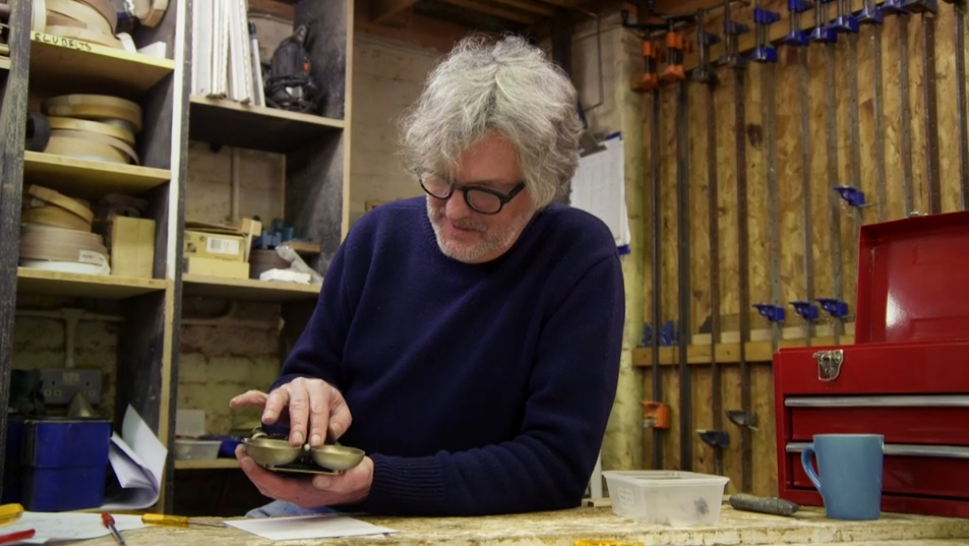
\includegraphics[width=0.75\textwidth]{TheReassembler}
    \caption{The Reassembler, S1E2}
\end{figure}

In this episode in particular, he was reassembling an old GPO phone 
(I believe that it was a 332, however it was never stated in the show, as far as I could tell),
and the part where he reassembled the dial assembly piqued my interest with how simple it was.
When the dial is rotating back to its original position, 
two contacts inside the assembly complete a circuit 10 times a second, 
with the amount of pulses equal to the number dialled (0 giving 10 pulses).\\
I immidiately thought of how easy that would be to interface to an arduino, 
by connecting one of the contacts to ground and the other to a digital pin, 
and activating the internal pullup resistor. This then became my primary idea, 
and all I had to do was get it signed off to start work.\\
One benefit that I had duringthis project was that my father worked in BT for many years,
and even though he had left, he still had several contacts, 
which meant that it was surprisingly easy to get hold of an old GPO phone.
I ended up recieving a 746, which is slightly different to the model in the TV show,
but still worked in the same way.\\

\begin{figure}[h]
    \centering
    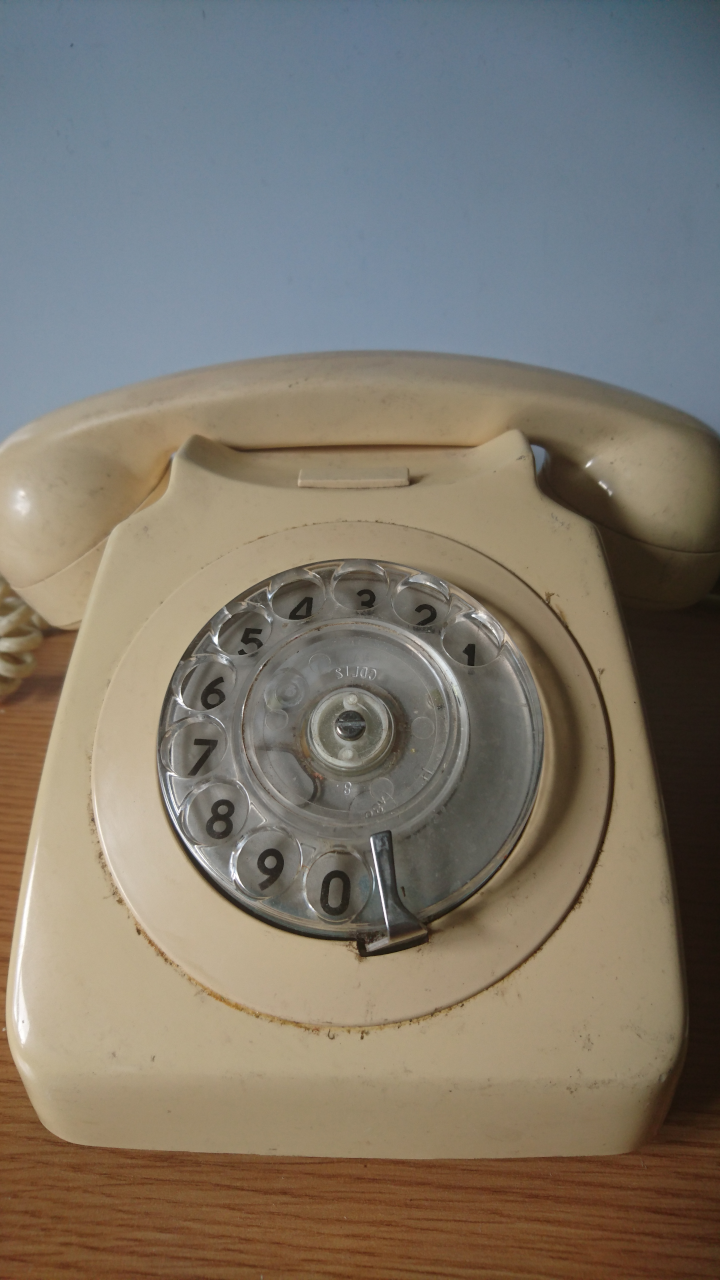
\includegraphics[width=0.25\textwidth]{PhoneFront}
    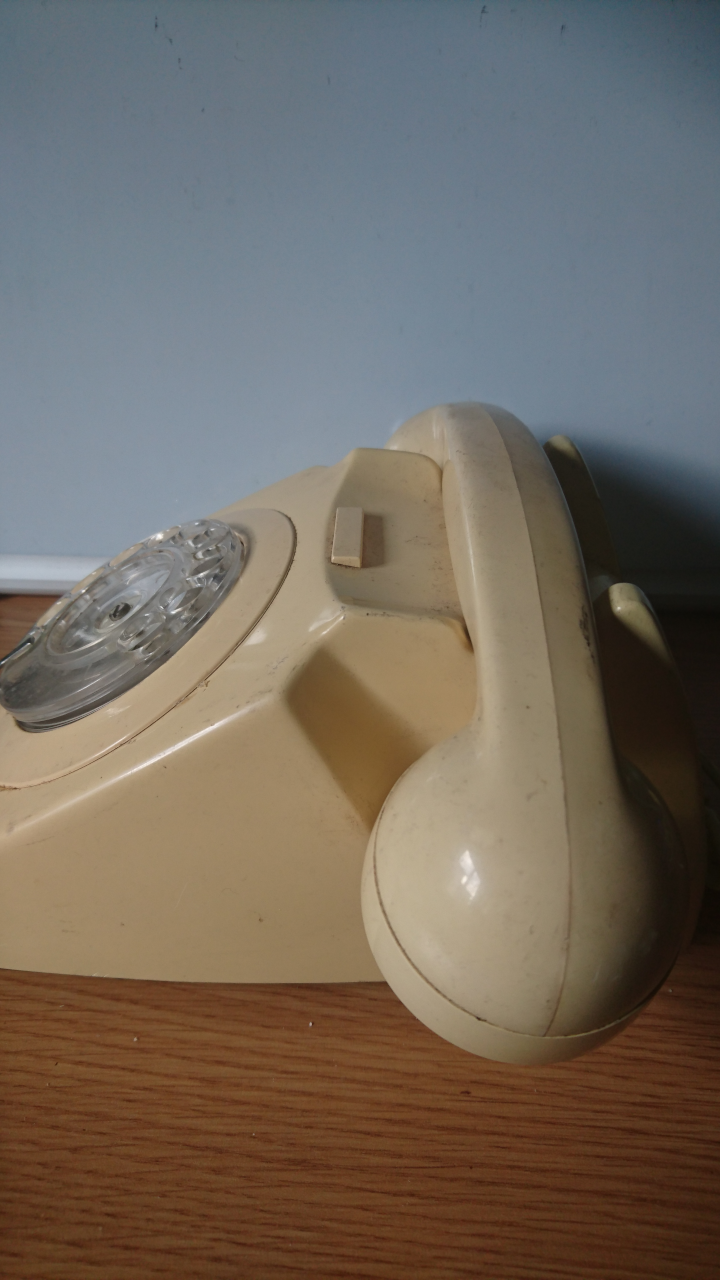
\includegraphics[width=0.25\textwidth]{PhoneSide}
    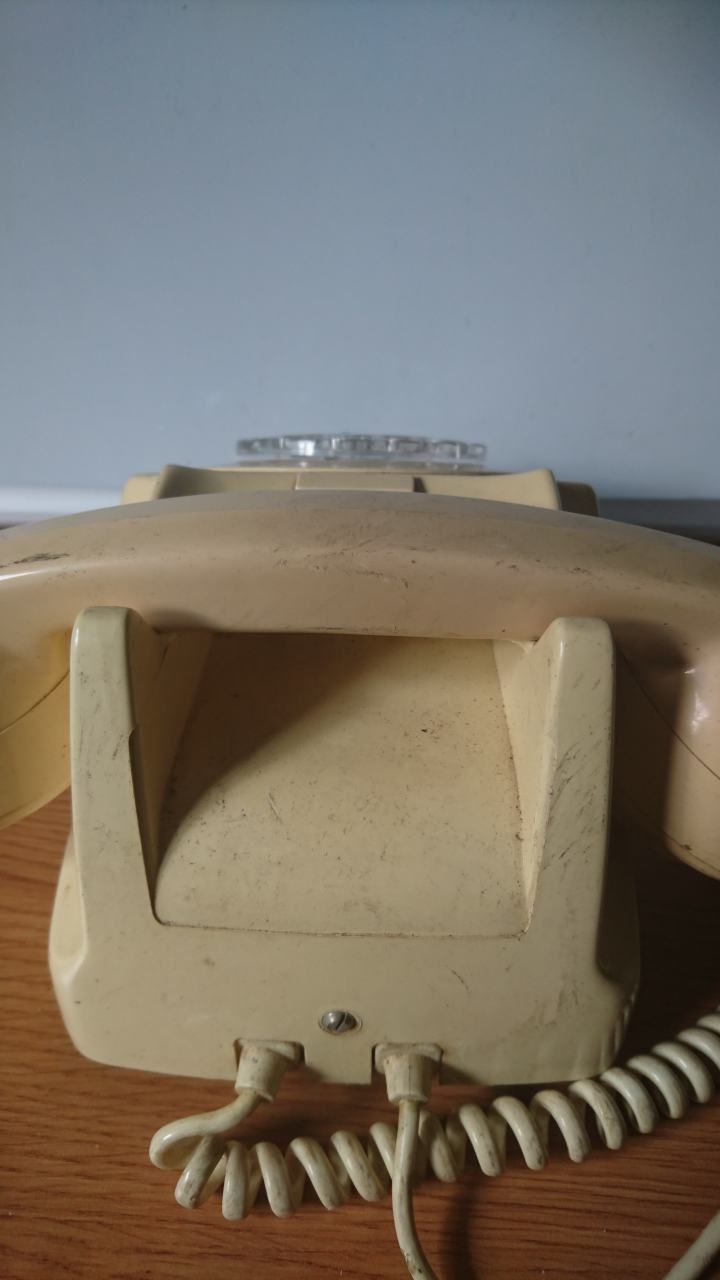
\includegraphics[width=0.25\textwidth]{PhoneBack}
    \caption{The phone as I recieved it. The dirt does not show up well on camera, but it is quite bad}
\end{figure}

When I recieved the phone, it was a little worse for wear,
however it was an older piece of technology, which meant that it was quite easy to service.
Removing one screw at the back allowed me to take off the top shell, which I then washed,
along with parts of the dial assembly. After that was done, 
the only remaing problem was that the dial would often stick, 
and not return to its resting position easily. 
I fixed this by adding a small amount of lubricant to the internal mechanism of the dial.\\
One interesting thing to note is that on the bottom of many GPO phones, there are very informative manufacturer markings. For example on the bottom of this phone, you can see "746F DFM 80/2".

\begin{figure}[h]
    \centering
    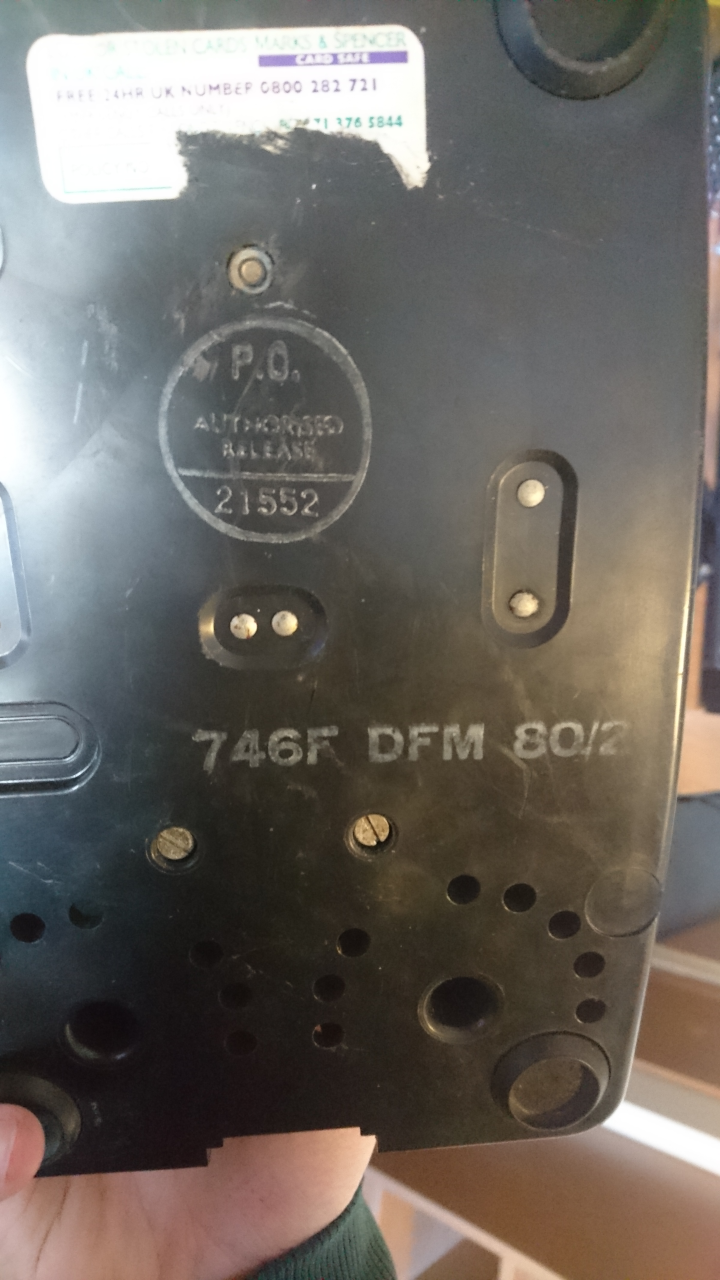
\includegraphics[width=0.25\textwidth]{PhoneBottom}
    \caption{The bottom of the phone, with the manufacturers marks visible}
\end{figure}

This specific code means that it is a 746, with only numbers on the dial, 
as opposed to letters and numbers, made by Denis Ferranti Meters Ltd., 
made in 1980 as part of production run 2. 
Denis Ferranti Meters Ltd is now known as Denis Ferranti Electronics, who are still in business, 
and they currently make PCBs for companies like BAE systems, the MOD and Perkins.\\

\FloatBarrier
\section{Hardware} %ii.  Hardware of the controller, including components
For the hardware, I initially thought that I would have to use a few extra components, 
but I ended up using just an arduino uno and a couple of wires. 
I knew that there would be an issue with switch bouncing, as I have encountered it in the past, 
so I was expecting to need an additional resistor and capacitor to debounce the dial contacts, 
however I ended up using a software solution instead, 
which was based off the example code provided in the arduino IDE. Aside from that, 
I only needed a couple of extra wires to get a ground, 
and the two signals from the switches that I wanted to listen to.

\begin{figure}[h]
    \centering
    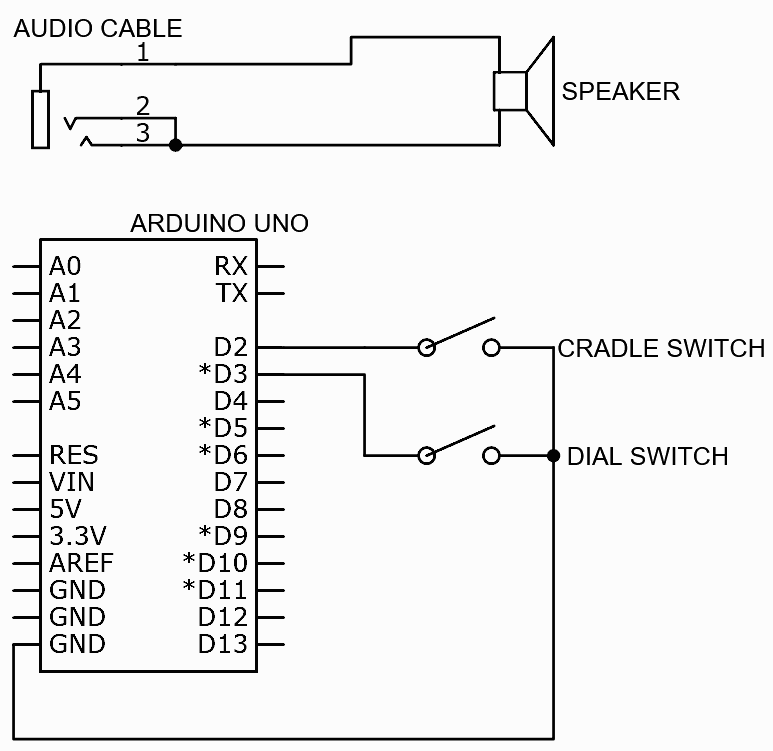
\includegraphics[width=0.5\textwidth]{CircuitDiagram}
    \caption{Circuit diagram of the phone circuitry. Note that the audio jack is a male cable in the actual controller, and that symbol has been used for convenience}
\end{figure}

\begin{figure}[h]
    \centering
    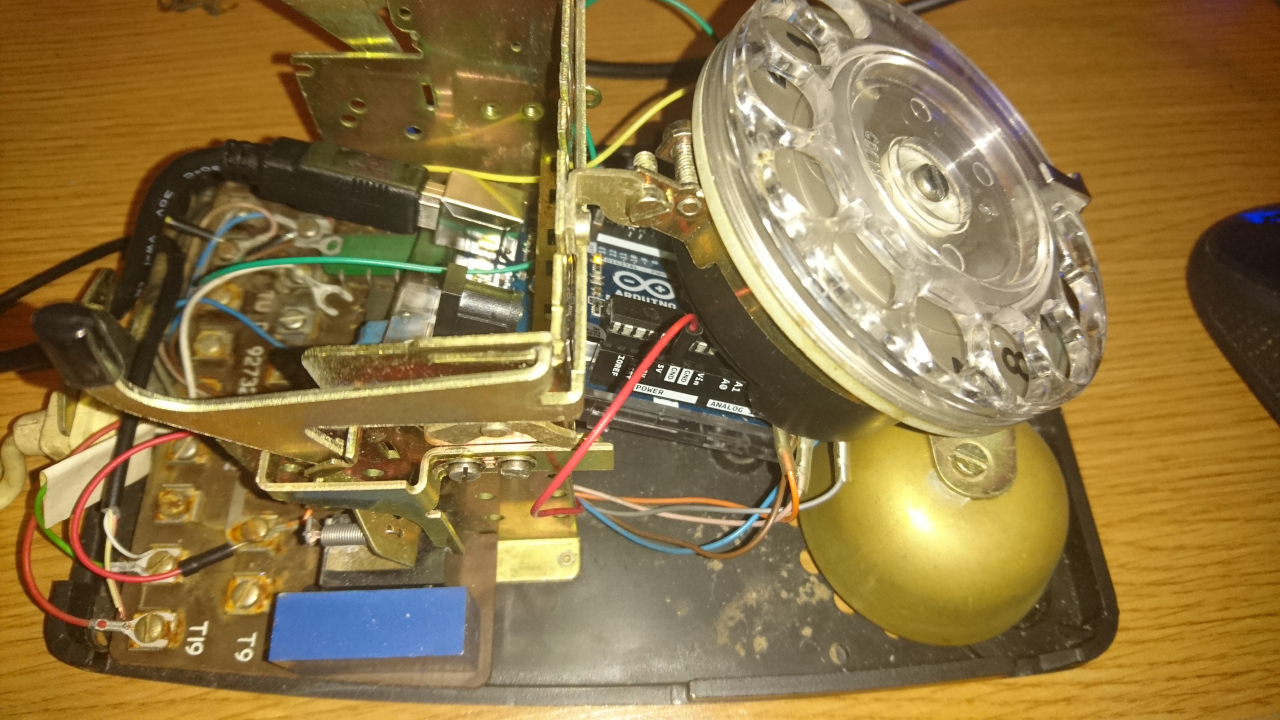
\includegraphics[width=0.5\textwidth]{PhoneInside}
    \caption{A inside view of the modified phone}
\end{figure}

One thing that I am a little annoyed at is that there wasnt quite enough space to fit the arduino in the top section, 
under the cradle switch, so I had to remove the bell mechanism and put the arduino underneath the dial. 
This meant that I couldnt use the bell mechanism. 
However I'm not sure that I would have used it in the final controller, 
since the current draw would likely have been too high for the usb port to handle, 
and would have required some external circuitry.
For playing the sounds back out of the phone, 
I guessed that the original speaker would use pretty much the same technology as a standard speaker of the current time, 
so I connected a headphone cable to it, and it worked perfectly. 
This meant that I didnt have to mess with the original handset at all, 
and could keep all the wiring in the bottom section. I used unity to actually play the audio, 
which saved me having to buy something like an Adafruit WAVTrigger, and do it all in hardware.

\FloatBarrier
\section{Software} %v.  Software design with UML Diagrams
The software design remained fairly constant through the entire project, 
with the arduino simply listening to the hardware, 
and sending the events back to the unity game (events such as "the handset waas picked up", 
"The user dialled a 3" etc.). This meant that I didn't have to code as much in C, 
a language I am not very confident in, and would have to code more in C\#, 
a language I am much more familiar with. 
I could also take advantage of a lot of the features of unity such as scriptable objects, 
which allowed me to write a single definition for a menu item, 
and then I could quickly make lots of them using the graphical editor, 
adding sound clips and child menu entries as needed.\\
One extra program I had to write was a small application to interface with the windows narrator,
so that I could feed it text and get back .wav files of that text being spoken.
This wasn't particularly hard, as C\# has the SpeechSynthesis namespace,
which allows full access to all installed narrator voices.

\FloatBarrier
\subsection{UML Diagrams}
\begin{figure}[h]
    \centering
    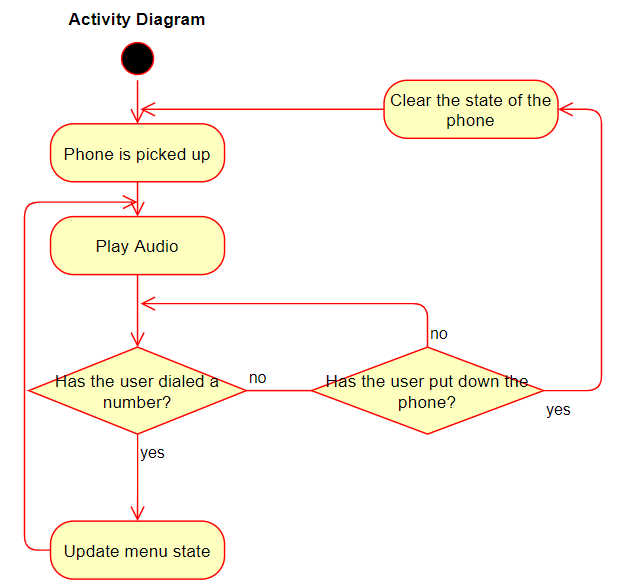
\includegraphics[width=0.5\textwidth]{ActivityDiagram}
    \caption{Activity Diagram}
\end{figure}

\begin{figure}[h]
    \centering
    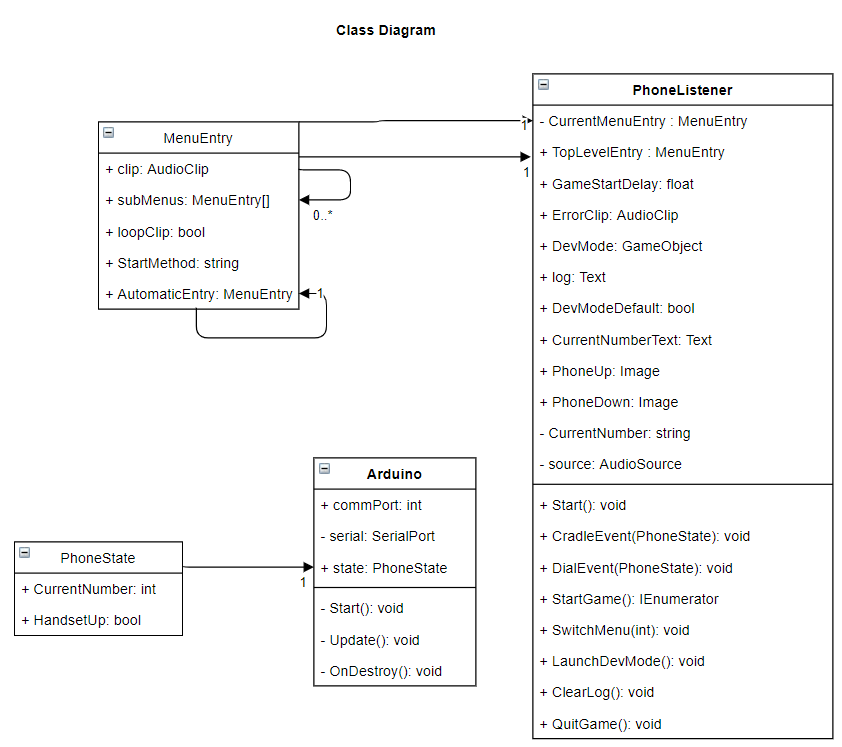
\includegraphics[width=0.75\textwidth]{ClassDiagram}
    \caption{Class Diagram}
\end{figure}

\begin{figure}[h]
    \centering
    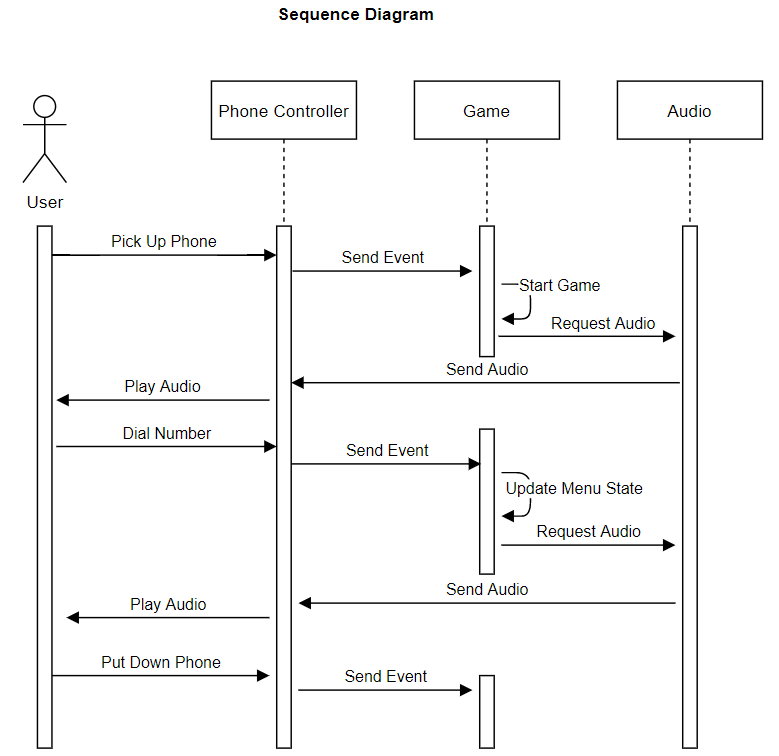
\includegraphics[width=0.5\textwidth]{SequenceDiagram}
    \caption{Sequence Diagram}
\end{figure}

\begin{figure}[h]
    \centering
    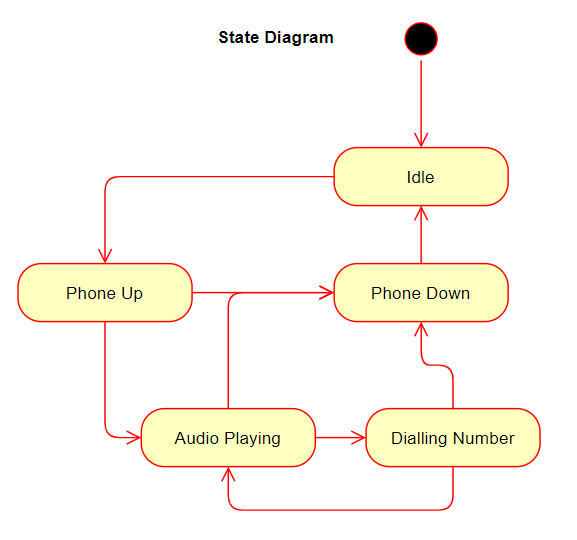
\includegraphics[width=0.5\textwidth]{StateDiagram}
    \caption{State Diagram}
\end{figure}

\begin{figure}[h]
    \centering
    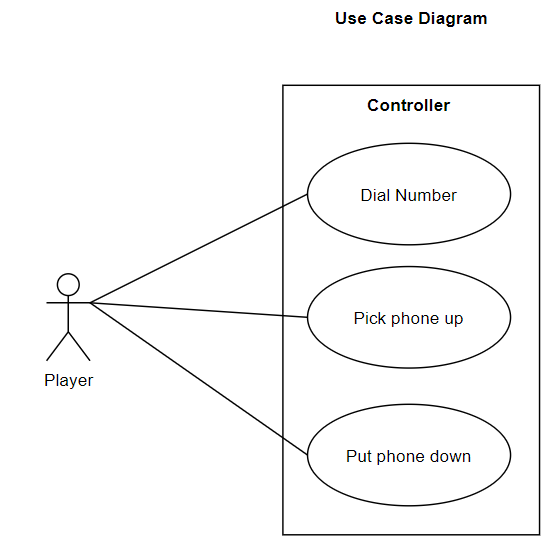
\includegraphics[width=0.5\textwidth]{UseCaseDiagram}
    \caption{Use Case Diagram}
\end{figure}

\FloatBarrier
\section{Concept} %iv.  The game/experience concept
The original concept of the experience was to be able to listen to phone calls that had been made on a small island,
and use the information in the calls to try and work out the story of what had happened to all the inhabitants of the island itself.
However, to make it more interesting, I wanted to only have one side of the conversation recorded,
and it be spoken by a synthesized voice. 
The in-game reason being that there was limited storage space availible, 
due to it being set in the 80's, when the phone was made. 
The out-of-game reason was that it enabled me to write a simple application to interface with windows narrator,
and churn out voice lines without having to hire voice actors. 
Also, I had just played Her Story at that point, which I had loved, 
and I wanted to somewhat re-create the experience.\\
In the story, Big Mines inc. has found evidence of high quality iron ore on the island, 
and wish to mine it, however the island holds a terrible force of evil that should never be unleashed.
Obviously, the mining company goes ahead and releases it, and terrible events ensue.

\FloatBarrier
\section{Reflection} %vi.  Reflection on the project
I feel that this project has gone remarkably smoothly, with only a few minor hiccups. 
Actually aquiring the phone took a little longer than I would have desired, 
which lead to a delay in properly starting the project, 
however I was still able to write the software at that point, so there weren't massive problems. 
The software had to be slightly re-designed at a couple of stages to accomodate new issues that I hadn't thought of at the start, 
however it also went decently smoothly.\\
The only real issue that I have is that while the idea may have worked out well in the hands of a team including a writer,
it was rather ambitious for a single programmer. 
The execution slightly falls flat with how I am using the voices, 
and I have found it difficult to write a vaguely good story without enough extra detail to make it interesting to try and find the important stuff.

\end{document}





